\documentclass[12pt,a4paper]{article}

% --- Cài đặt cơ bản ---
\usepackage[utf8]{inputenc} % Hỗ trợ gõ tiếng Việt
\usepackage[T5]{fontenc}    % Mã hóa font cho tiếng Việt
\usepackage[vietnamese]{babel} % Gói hỗ trợ ngôn ngữ tiếng Việt
\usepackage{geometry}       % Điều chỉnh lề trang
\geometry{a4paper, margin=2.5cm, top=3cm, bottom=3cm} % Cài đặt lề chuẩn

% --- Gói cho typography và định dạng chuyên nghiệp ---
\usepackage{setspace}       % Điều chỉnh khoảng cách dòng (ví dụ: 1.5 lines)
\usepackage{titlesec}       % Tùy chỉnh định dạng tiêu đề các phần/chương
\usepackage{tocloft}        % Tùy chỉnh mục lục và danh sách bảng/hình
\usepackage{caption}        % Tùy chỉnh caption cho bảng và hình ảnh
\usepackage{subcaption}     % Hỗ trợ subfigure và subcaption (nếu cần nhiều hình trong 1 caption)
\usepackage{ragged2e}       % Cho phép căn đều văn bản (justifying), tốt hơn \justify
\usepackage{booktabs}       % Cho bảng đẹp hơn với đường kẻ chuyên nghiệp (\toprule, \midrule, \bottomrule)
\usepackage{enumitem}       % Tùy chỉnh danh sách (itemize, enumerate)
\usepackage{microtype}      % Cải thiện kiểu chữ và căn chữ
\usepackage{pifont}         % Bộ biểu tượng cho bullet tùy chỉnh
\usepackage{float}          % Cho phép vị trí bảng/hình ảnh chính xác hơn [H]
\usepackage{tabularx}       % Bảng có thể tự động điều chỉnh chiều rộng cột
\usepackage{longtable}      % Cho bảng dài trải dài nhiều trang
\usepackage{graphicx}       % Thêm gói này để chèn ảnh

% --- Gói cho toán học (giữ lại nếu có dùng công thức toán) ---
\usepackage{amsmath}        % Các môi trường toán học mở rộng (align, equation, v.v.)
\usepackage{amssymb}        % Các ký hiệu toán học bổ sung

% --- Gói cho header/footer ---
\usepackage{fancyhdr}       % Tùy chỉnh header và footer

% --- Gói cho màu sắc ---
\usepackage{xcolor}         % Định nghĩa và sử dụng màu sắc
\usepackage[most]{tcolorbox} % Tạo khung màu chuyên nghiệp
\definecolor{darkblue}{RGB}{0,82,155}   % Màu xanh đậm cho tiêu đề
\definecolor{darkgreen}{RGB}{0,128,0}   % Màu xanh lá đậm cho URL

% --- Tuỳ chỉnh danh sách ---
\setlist[itemize]{leftmargin=1cm,label=\textcolor{darkblue}{\small\textbullet}}

% --- Khung nổi bật cho phân tích rủi ro ---
\newtcolorbox{riskbox}{
    colback=white,
    colframe=darkblue,
    fonttitle=\bfseries,
    coltitle=darkblue,
    boxrule=0.5pt,
    arc=2mm,
    left=4pt,
    right=4pt,
    top=4pt,
    bottom=4pt,
}

% --- Cấu hình định dạng tiêu đề ---
% Sử dụng \normalfont để đảm bảo font không bị ảnh hưởng bởi các lệnh trước đó
\titleformat{\section}{\normalfont\Large\bfseries\color{darkblue}}{\thesection}{1em}{}
\titleformat{\subsection}{\normalfont\large\bfseries\color{darkblue}}{\thesubsection}{1em}{}
\titleformat{\subsubsection}{\normalfont\normalsize\bfseries\color{darkblue}}{\thesubsubsection}{1em}{}

% --- Cấu hình spacing tối ưu ---
\onehalfspacing             % Khoảng cách dòng 1.5
\setlength{\parindent}{0.5cm} % Thụt đầu dòng 0.5cm
\setlength{\parskip}{6pt}   % Khoảng cách giữa các đoạn văn
\setlength{\arrayrulewidth}{0.5pt}  % Độ dày đường viền bảng
%\renewcommand{\arraystretch}{1.2}   % ĐÃ LOẠI BỎ/ĐIỀU CHỈNH: Khoảng cách dòng trong bảng (để về mặc định)

% --- Cấu hình hyperref (đặt cuối cùng trong preamble) ---
\usepackage{hyperref}
\hypersetup{
    colorlinks=true,        % Màu cho các liên kết
    linkcolor=darkblue,     % Màu của các liên kết nội bộ (mục lục, hình, bảng)
    filecolor=magenta,      % Màu của liên kết đến file cục bộ
    urlcolor=darkgreen,     % Màu của URL
    citecolor=darkblue,     % Màu của các trích dẫn
    pdftitle={Báo cáo giữa kỳ - Dự án Smart Canteen AR}, % Tiêu đề hiển thị trong thuộc tính PDF
    pdfauthor={Nhóm 5 - Trường Đại học Khoa học Tự nhiên TPHCM}, % Tác giả hiển thị trong thuộc tính PDF
    pdfsubject={Dự án Khởi nghiệp Đổi mới Sáng tạo}, % Chủ đề PDF
    pdfkeywords={Smart Canteen, AR, Thực tế tăng cường, Căng tin thông minh}, % Từ khóa PDF
    bookmarks=true,         % Tạo bookmark trong PDF
    bookmarksopen=true,     % Mở bookmark khi mở PDF
    bookmarksnumbered=true, % Đánh số bookmark
    pdfstartview={FitH}     % Chế độ xem khi mở PDF (Fit to Width)
}

% --- Định nghĩa tiêu đề và tác giả cho trang bìa ---
% Sử dụng \vfill để căn giữa theo chiều dọc
\title{
    \vspace{-1cm} % Điều chỉnh vị trí tiêu đề lên trên một chút
    {\huge\textbf{\color{darkblue}BÁO CÁO GIỮA KỲ}} \\[0.5cm]
    {\LARGE\textbf{\color{darkblue}DỰ ÁN SMART CANTEEN AR}} \\[0.3cm]
    {\large\textit{Ứng dụng thực tế tăng cường trong căng tin thông minh}}
}

\author{
    \begin{tabular}{c}
        \textbf{\large DỰ ÁN KHỞI NGHIỆP ĐỔI MỚI SÁNG TẠO} \\[0.5cm]
        \textbf{NHÓM THỰC HIỆN: NHÓM 5} \\[0.3cm]
        \begin{tabular}{@{}l@{\hspace{2cm}}l@{}} % Sử dụng @{} để bỏ khoảng trống ở đầu/cuối hàng
            \textbf{1.} Hồ Sĩ Phú (Nhóm trưởng) & \textbf{4.} Lê Quang Bảo Trung \\
            \textbf{2.} Phạm Cao Bằng & \textbf{5.} Trần Thái Nguyên \\
            \textbf{3.} Phạm Hùng Tiến & \\
        \end{tabular} \\[0.5cm]
        \textbf{ĐƠN VỊ THỰC HIỆN} \\
        \textit{Trường Đại học Khoa học Tự nhiên - ĐHQG TPHCM} \\[0.3cm]
        \textbf{Thành phố Hồ Chí Minh, năm 2025}
    \end{tabular}
}

\date{} % Bỏ ngày tháng để không hiển thị ngày mặc định

\begin{document}

% --- Trang tiêu đề ---
\begin{titlepage}
    \thispagestyle{empty} % Xóa header/footer cho trang tiêu đề
    \centering           % Căn giữa nội dung trang bìa

    % Có thể thêm logo nếu có (ví dụ: \includegraphics[width=4cm]{../figures/logo.png}\\[1cm])
    % \vspace*{1cm} % Tùy chỉnh khoảng trống nếu cần

    \maketitle % Lệnh hiển thị Title và Author đã định nghĩa ở trên

    \vfill % Đẩy phần nội dung phụ xuống dưới cùng trang
    % Thông tin bổ sung ở cuối trang bìa
    \begin{tabular}{@{}l@{\hspace{1cm}}l@{}}
        \textbf{Lớp:} & 24DTV\_DKD2 \\
        \textbf{Học kỳ:} & 3, năm học 2024-2025 \\
    \end{tabular}
    \vspace{1cm} % Khoảng cách từ thông tin bổ sung đến cuối trang
\end{titlepage}

% --- Đặt lại page style cho các trang tiếp theo ---
\newpage
\setcounter{page}{1} % Đặt lại số trang về 1 cho phần nội dung chính
% Cấu hình fancyhdr cho các trang nội dung
\pagestyle{fancy}
\fancyhf{} % Xóa tất cả header/footer mặc định
\fancyhead[L]{\textit{Smart Canteen AR - Báo cáo giữa kỳ}} % Header bên trái
\fancyhead[R]{\textit{Nhóm 5}} % Header bên phải
\fancyfoot[C]{\thepage} % Số trang ở giữa footer
\renewcommand{\headrulewidth}{0.4pt} % Độ dày đường kẻ dưới header
\renewcommand{\footrulewidth}{0pt}   % Bỏ đường kẻ trên footer

% --- Áp dụng căn đều cho toàn bộ tài liệu ---
\justifying % Căn đều văn bản, sử dụng từ gói ragged2e

% --- Mục lục ---
\tableofcontents
\newpage

% --- Danh sách bảng ---
\listoftables
\newpage

% --- Danh sách hình ảnh ---
\listoffigures
\newpage

% --- Danh mục viết tắt ---
\section*{Danh mục viết tắt} % Sử dụng * để không đánh số phần này
\addcontentsline{toc}{section}{Danh mục viết tắt} % Thêm vào mục lục thủ công

\begin{table}[H]
\centering
\caption{Danh mục viết tắt}
\label{tab:abbreviations}
\begin{tabular}{@{}p{3cm}@{\hspace{1cm}}p{10cm}@{}} % p{} cho phép xuống dòng
    \toprule % Đường kẻ trên cùng (từ booktabs)
    \textbf{Viết tắt} & \textbf{Nghĩa đầy đủ} \\
    \midrule % Đường kẻ giữa (từ booktabs)
    AR & Augmented Reality (Thực tế tăng cường) \\
    MVP & Minimum Viable Product (Sản phẩm khả thi tối thiểu) \\
    F\&B & Food \& Beverage (Thực phẩm và Đồ uống) \\
    TAM & Total Addressable Market (Thị trường tổng thể có thể phục vụ) \\
    POS & Point of Sale (Điểm bán hàng) \\
    UI/UX & User Interface / User Experience (Giao diện người dùng / Trải nghiệm người dùng) \\
    R\&D & Research and Development (Nghiên cứu và phát triển) \\
    ĐMST & Đổi mới sáng tạo \\
    API & Application Programming Interface (Giao diện lập trình ứng dụng) \\
    JSON & JavaScript Object Notation (Định dạng dữ liệu JavaScript) \\
    QR & Quick Response (Phản hồi nhanh) \\
    SMS & Short Message Service (Dịch vụ tin nhắn ngắn) \\
    SMTP & Simple Mail Transfer Protocol (Giao thức truyền thư đơn giản) \\
    \bottomrule % Đường kẻ dưới cùng (từ booktabs)
\end{tabular}
\end{table}

\newpage

% --- Nội dung chính của báo cáo ---
\section{Tổng quan dự án}

\subsection{Tên dự án}
\textbf{Smart Canteen AR} - Hệ thống căng tin thông minh tích hợp công nghệ thực tế tăng cường.
\subsection{Tầm nhìn}
Smart Canteen AR hướng tới trở thành \textbf{hệ thống căng tin thông minh hàng đầu} tại Việt Nam, tiên phong trong việc ứng dụng công nghệ thực tế tăng cường (AR) để:

\begin{itemize}[leftmargin=1cm]
    \item Nâng cao trải nghiệm toàn diện của người dùng trong việc khám phá, đặt món và tương tác với thực đơn
    \item Tối ưu hóa triệt để quy trình quản lý vận hành cho các căng tin
    \item Góp phần thúc đẩy chuyển đổi số trong ngành dịch vụ ăn uống
\end{itemize}

\subsection{Sứ mệnh}
Cung cấp một \textbf{nền tảng đặt món trực tuyến tiên tiến}, dễ sử dụng, minh bạch và hiệu quả, nhằm:

\begin{itemize}[leftmargin=1cm]
    \item \textbf{Đối với người dùng}: Mang lại trải nghiệm ẩm thực tiện lợi, trực quan và thú vị thông qua công nghệ AR
    \item \textbf{Đối với căng tin}: Hỗ trợ tối ưu hóa hoạt động, quản lý thực đơn, đơn hàng và doanh thu một cách chính xác, hiệu quả
    \item \textbf{Đối với xã hội}: Góp phần nâng cao chất lượng dịch vụ ăn uống tập thể và thúc đẩy ứng dụng công nghệ 4.0
\end{itemize}

\section{Ý tưởng chính của dự án}

Smart Canteen AR là một \textbf{hệ thống mô phỏng căng tin trực tuyến toàn diện}, được xây dựng với kiến trúc hiện đại và công nghệ tiên tiến:

\subsection{Kiến trúc hệ thống}
\begin{itemize}[leftmargin=1cm]
    \item \textbf{Frontend}: Giao diện người dùng hiện đại được phát triển bằng React
    \item \textbf{Backend}: Hệ thống máy chủ mạnh mẽ sử dụng Node.js
    \item \textbf{Công nghệ AR}: Tích hợp thư viện \texttt{<model-viewer>} để hiển thị mô hình 3D
    \item \textbf{Cơ sở dữ liệu}: Lưu trữ dữ liệu trong các file JSON để dễ dàng triển khai và quản lý
\end{itemize}

% --- VỊ TRÍ THÊM HÌNH ẢNH: KIẾN TRÚC HỆ THỐNG ---
\begin{figure}[H]
    \centering
    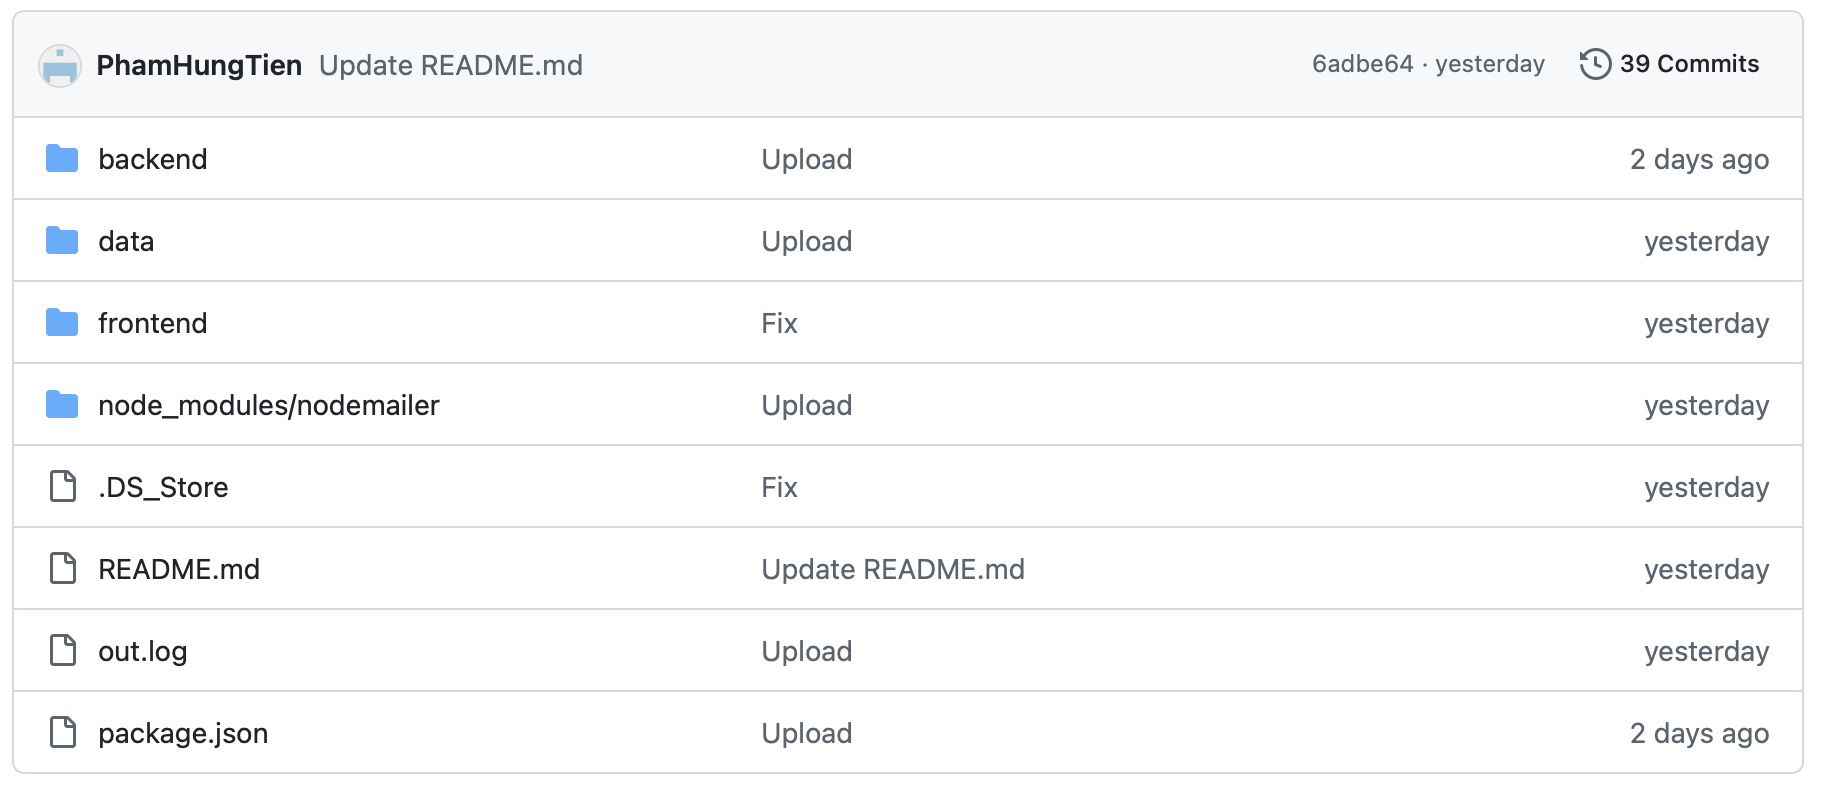
\includegraphics[width=0.8\textwidth]{../figures/kien_truc_he_thong.png} % Thay thế bằng tên file ảnh của bạn
    \caption{Sơ đồ kiến trúc hệ thống Smart Canteen AR}
    \label{fig:kien_truc_he_thong}
\end{figure}

\subsection{Điểm đột phá công nghệ}
\textbf{Tính năng AR độc đáo}: Người dùng có thể xem mô hình 3D của món ăn trực tiếp trên cả điện thoại và máy tính trước khi đặt hàng, mang lại trải nghiệm trực quan và hấp dẫn chưa từng có.

% --- VỊ TRÍ THÊM HÌNH ẢNH: MINH HỌA TÍNH NĂNG AR ---
\begin{figure}[H]
    \centering
    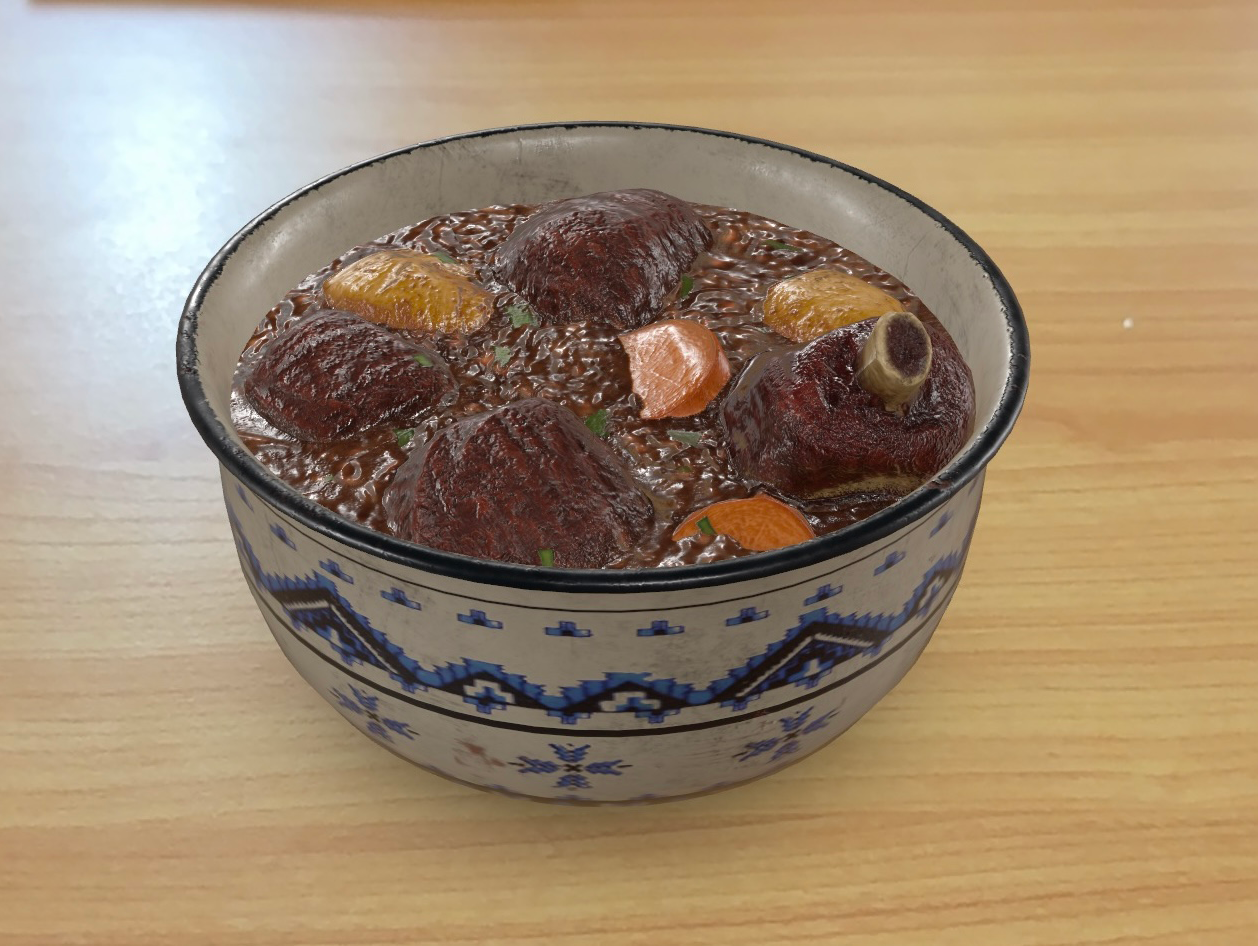
\includegraphics[width=\textwidth]{../figures/minh_hoa_ar_mon_an.png} % Thay thế bằng tên file ảnh của bạn
    \caption{Minh họa người dùng xem món ăn bằng công nghệ Thực tế tăng cường (AR)}
    \label{fig:ar_food_view}
\end{figure}

\subsection{Chức năng chính}

\subsubsection{Dành cho người dùng cuối}
\begin{itemize}[leftmargin=1cm]
    \item \textbf{Quản lý tài khoản}:
        \begin{itemize}[leftmargin=0.5cm]
            \item Đăng ký tài khoản mới tại \texttt{/signup} và đăng nhập tại \texttt{/login}
            \item Hỗ trợ quên mật khẩu và đổi mật khẩu
            \item Xác nhận email tự động sau khi đăng ký
        \end{itemize}
\begin{figure}[H]
    \centering
    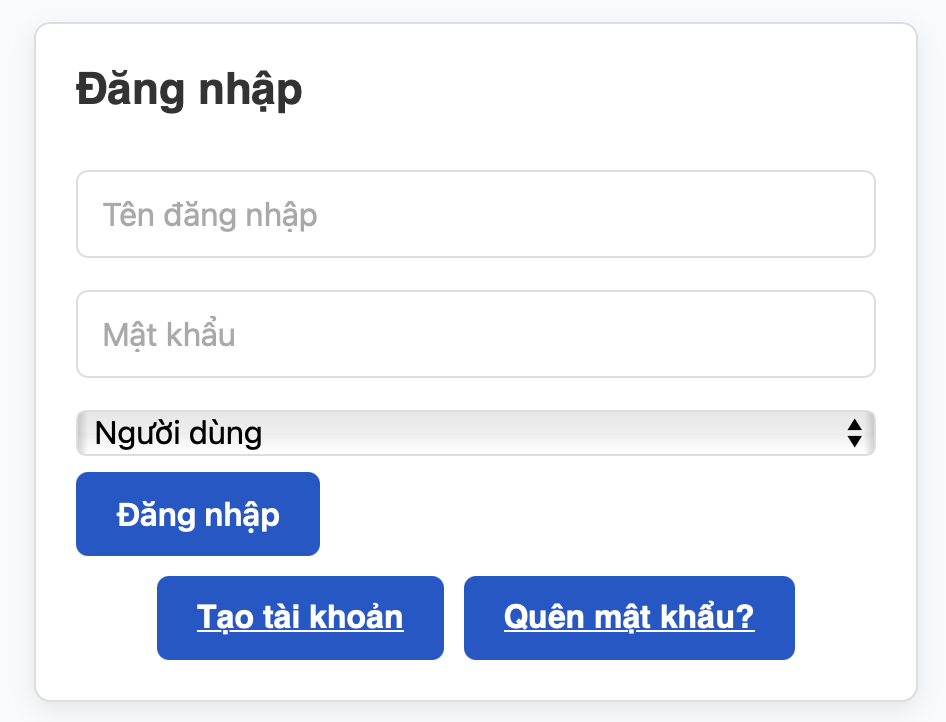
\includegraphics[width=0.9\textwidth]{../figures/ui_user_dang_nhap_dang_ky.png} % Thay thế bằng tên file ảnh của bạn
    \caption{Giao diện đăng nhập và đăng ký người dùng}
    \label{fig:ui_user_login_signup}
\end{figure}

    \item \textbf{Đặt món thông minh}:
        \begin{itemize}[leftmargin=0.5cm]
            \item Xem thực đơn với mô hình 3D tương tác (AR)
            \item Thêm món vào giỏ hàng và chọn thời gian lấy món
            \item Giới hạn thông minh: tối đa 5 đơn/khung 15 phút để tránh quá tải
            \item Thanh toán đa dạng: MoMo, VietQR
            \item Hệ thống thông báo email nhắc nhở (30 phút và 10 phút trước) với liên kết hủy đơn
        \end{itemize}
\begin{figure}[H]
    \centering
    \includegraphics[width=0.9\textwidth]{../figures/ui_user_thuc_don.png} % Thay thế bằng tên file ảnh của bạn
    \caption{Giao diện thực đơn và chi tiết món ăn của người dùng}
    \label{fig:ui_user_menu}
\end{figure}
\begin{figure}[H]
    \centering
    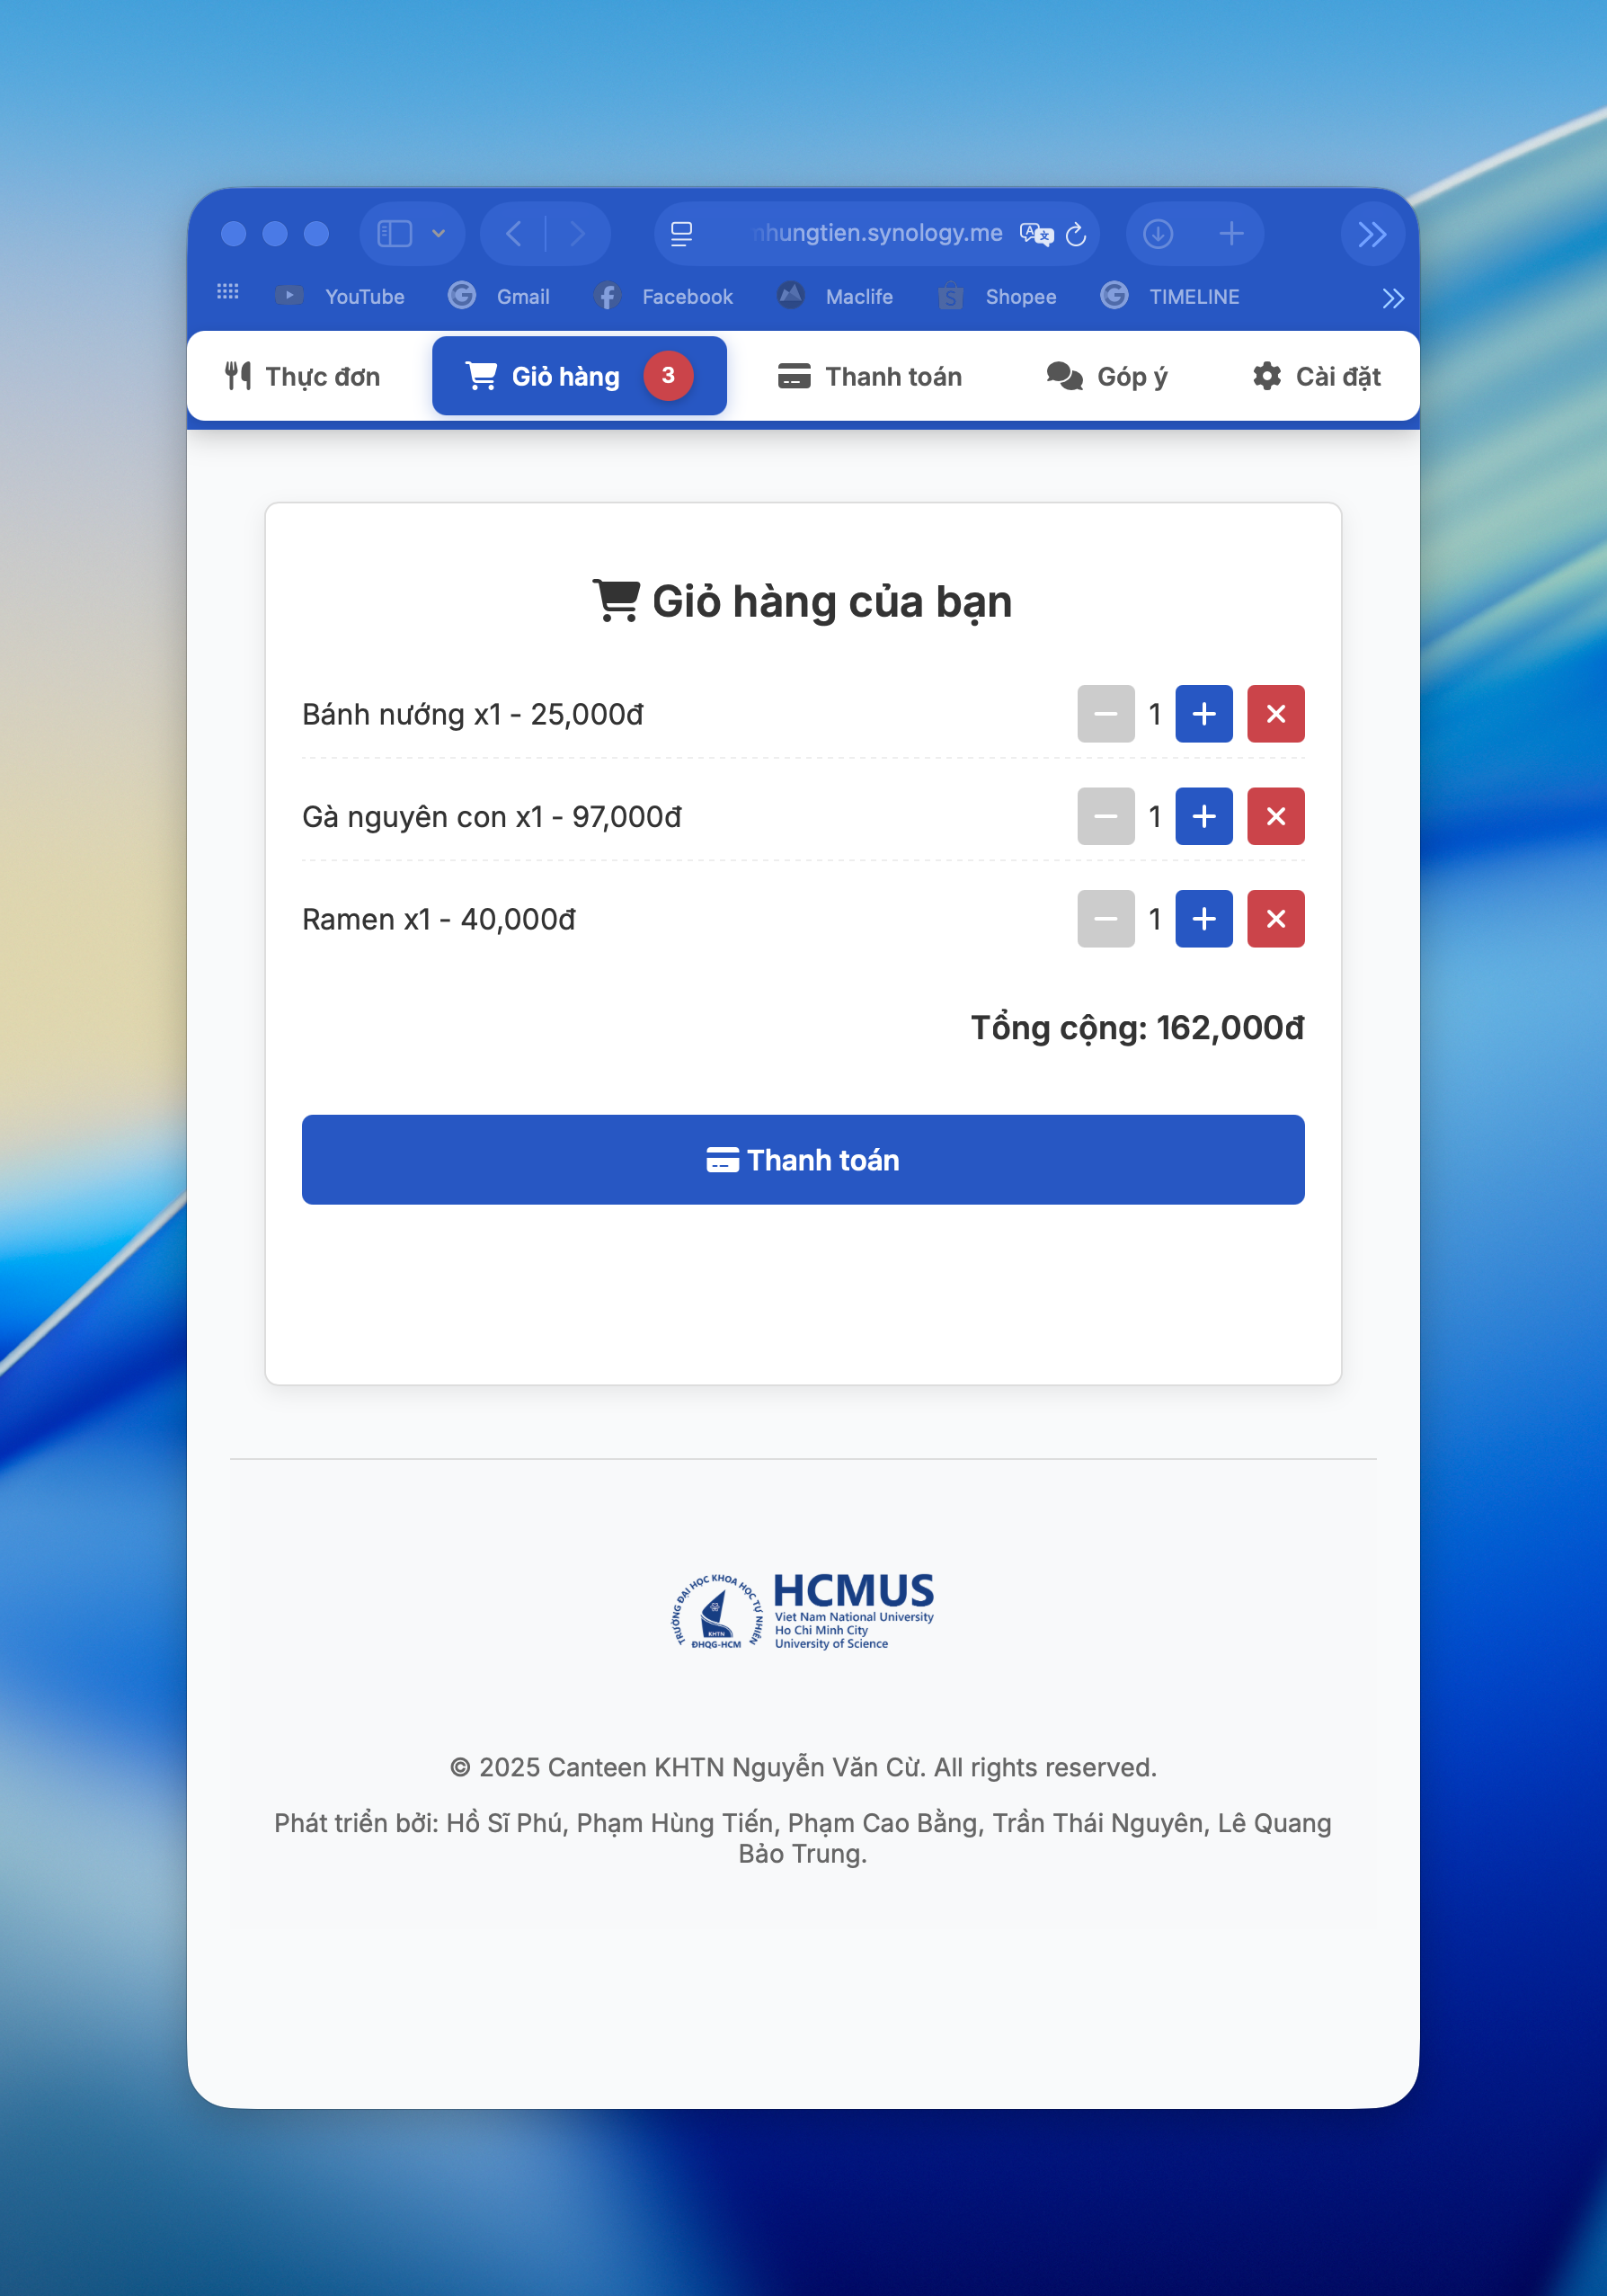
\includegraphics[width=0.9\textwidth]{../figures/ui_user_gio_hang_thanh_toan.png} % Thay thế bằng tên file ảnh của bạn
    \caption{Giao diện giỏ hàng và thanh toán (MoMo, VietQR) của người dùng}
    \label{fig:ui_user_cart_payment}
\end{figure}

    \item \textbf{Tương tác và phản hồi}:
        \begin{itemize}[leftmargin=0.5cm]
            \item Đánh giá món ăn bằng hệ thống sao và nhận xét
            \item Góp ý trực tiếp qua hệ thống
        \end{itemize}
\begin{figure}[H]
    \centering
    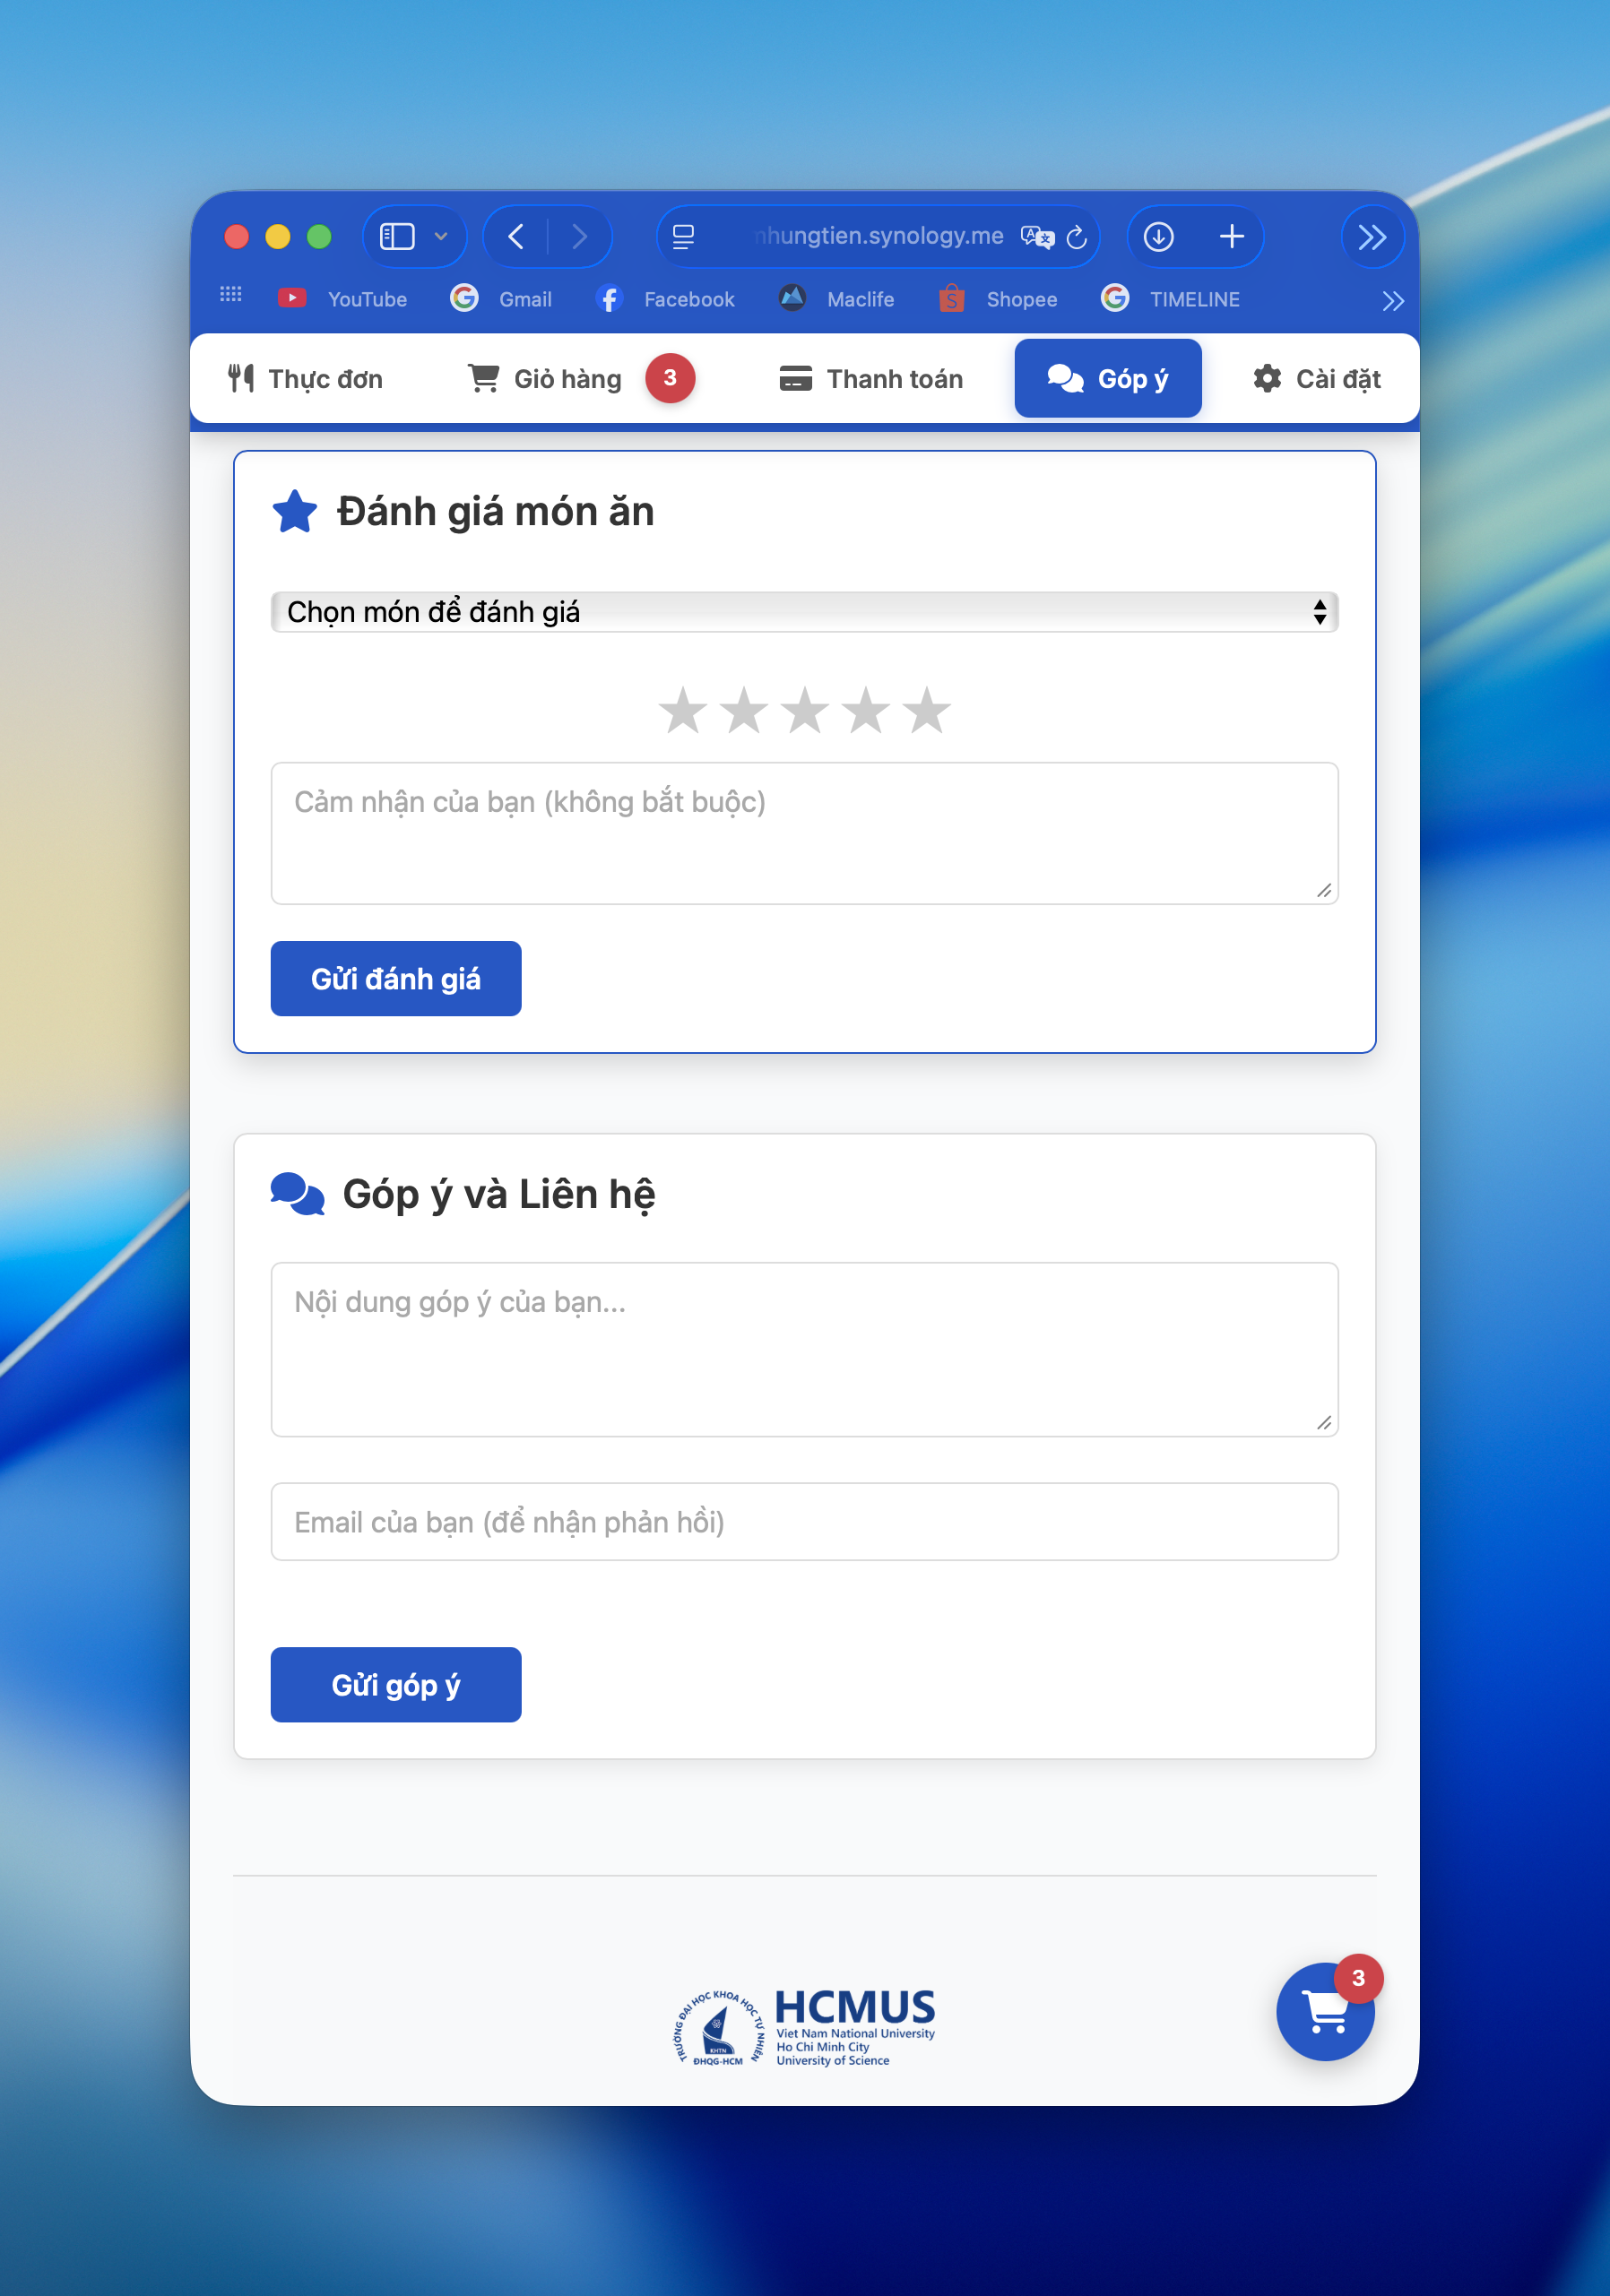
\includegraphics[width=0.9\textwidth]{../figures/ui_user_danh_gia_gop_y.png} % Thay thế bằng tên file ảnh của bạn
    \caption{Giao diện đánh giá món ăn và góp ý từ người dùng}
    \label{fig:ui_user_feedback}
\end{figure}

    \item \textbf{Cài đặt cá nhân}:
        \begin{itemize}[leftmargin=0.5cm]
            \item Thay đổi thông tin cá nhân
            \item Bật/tắt chế độ tối (Dark mode)
            \item Chọn ngôn ngữ (Việt/Anh)
        \end{itemize}
\begin{figure}[H]
    \centering
    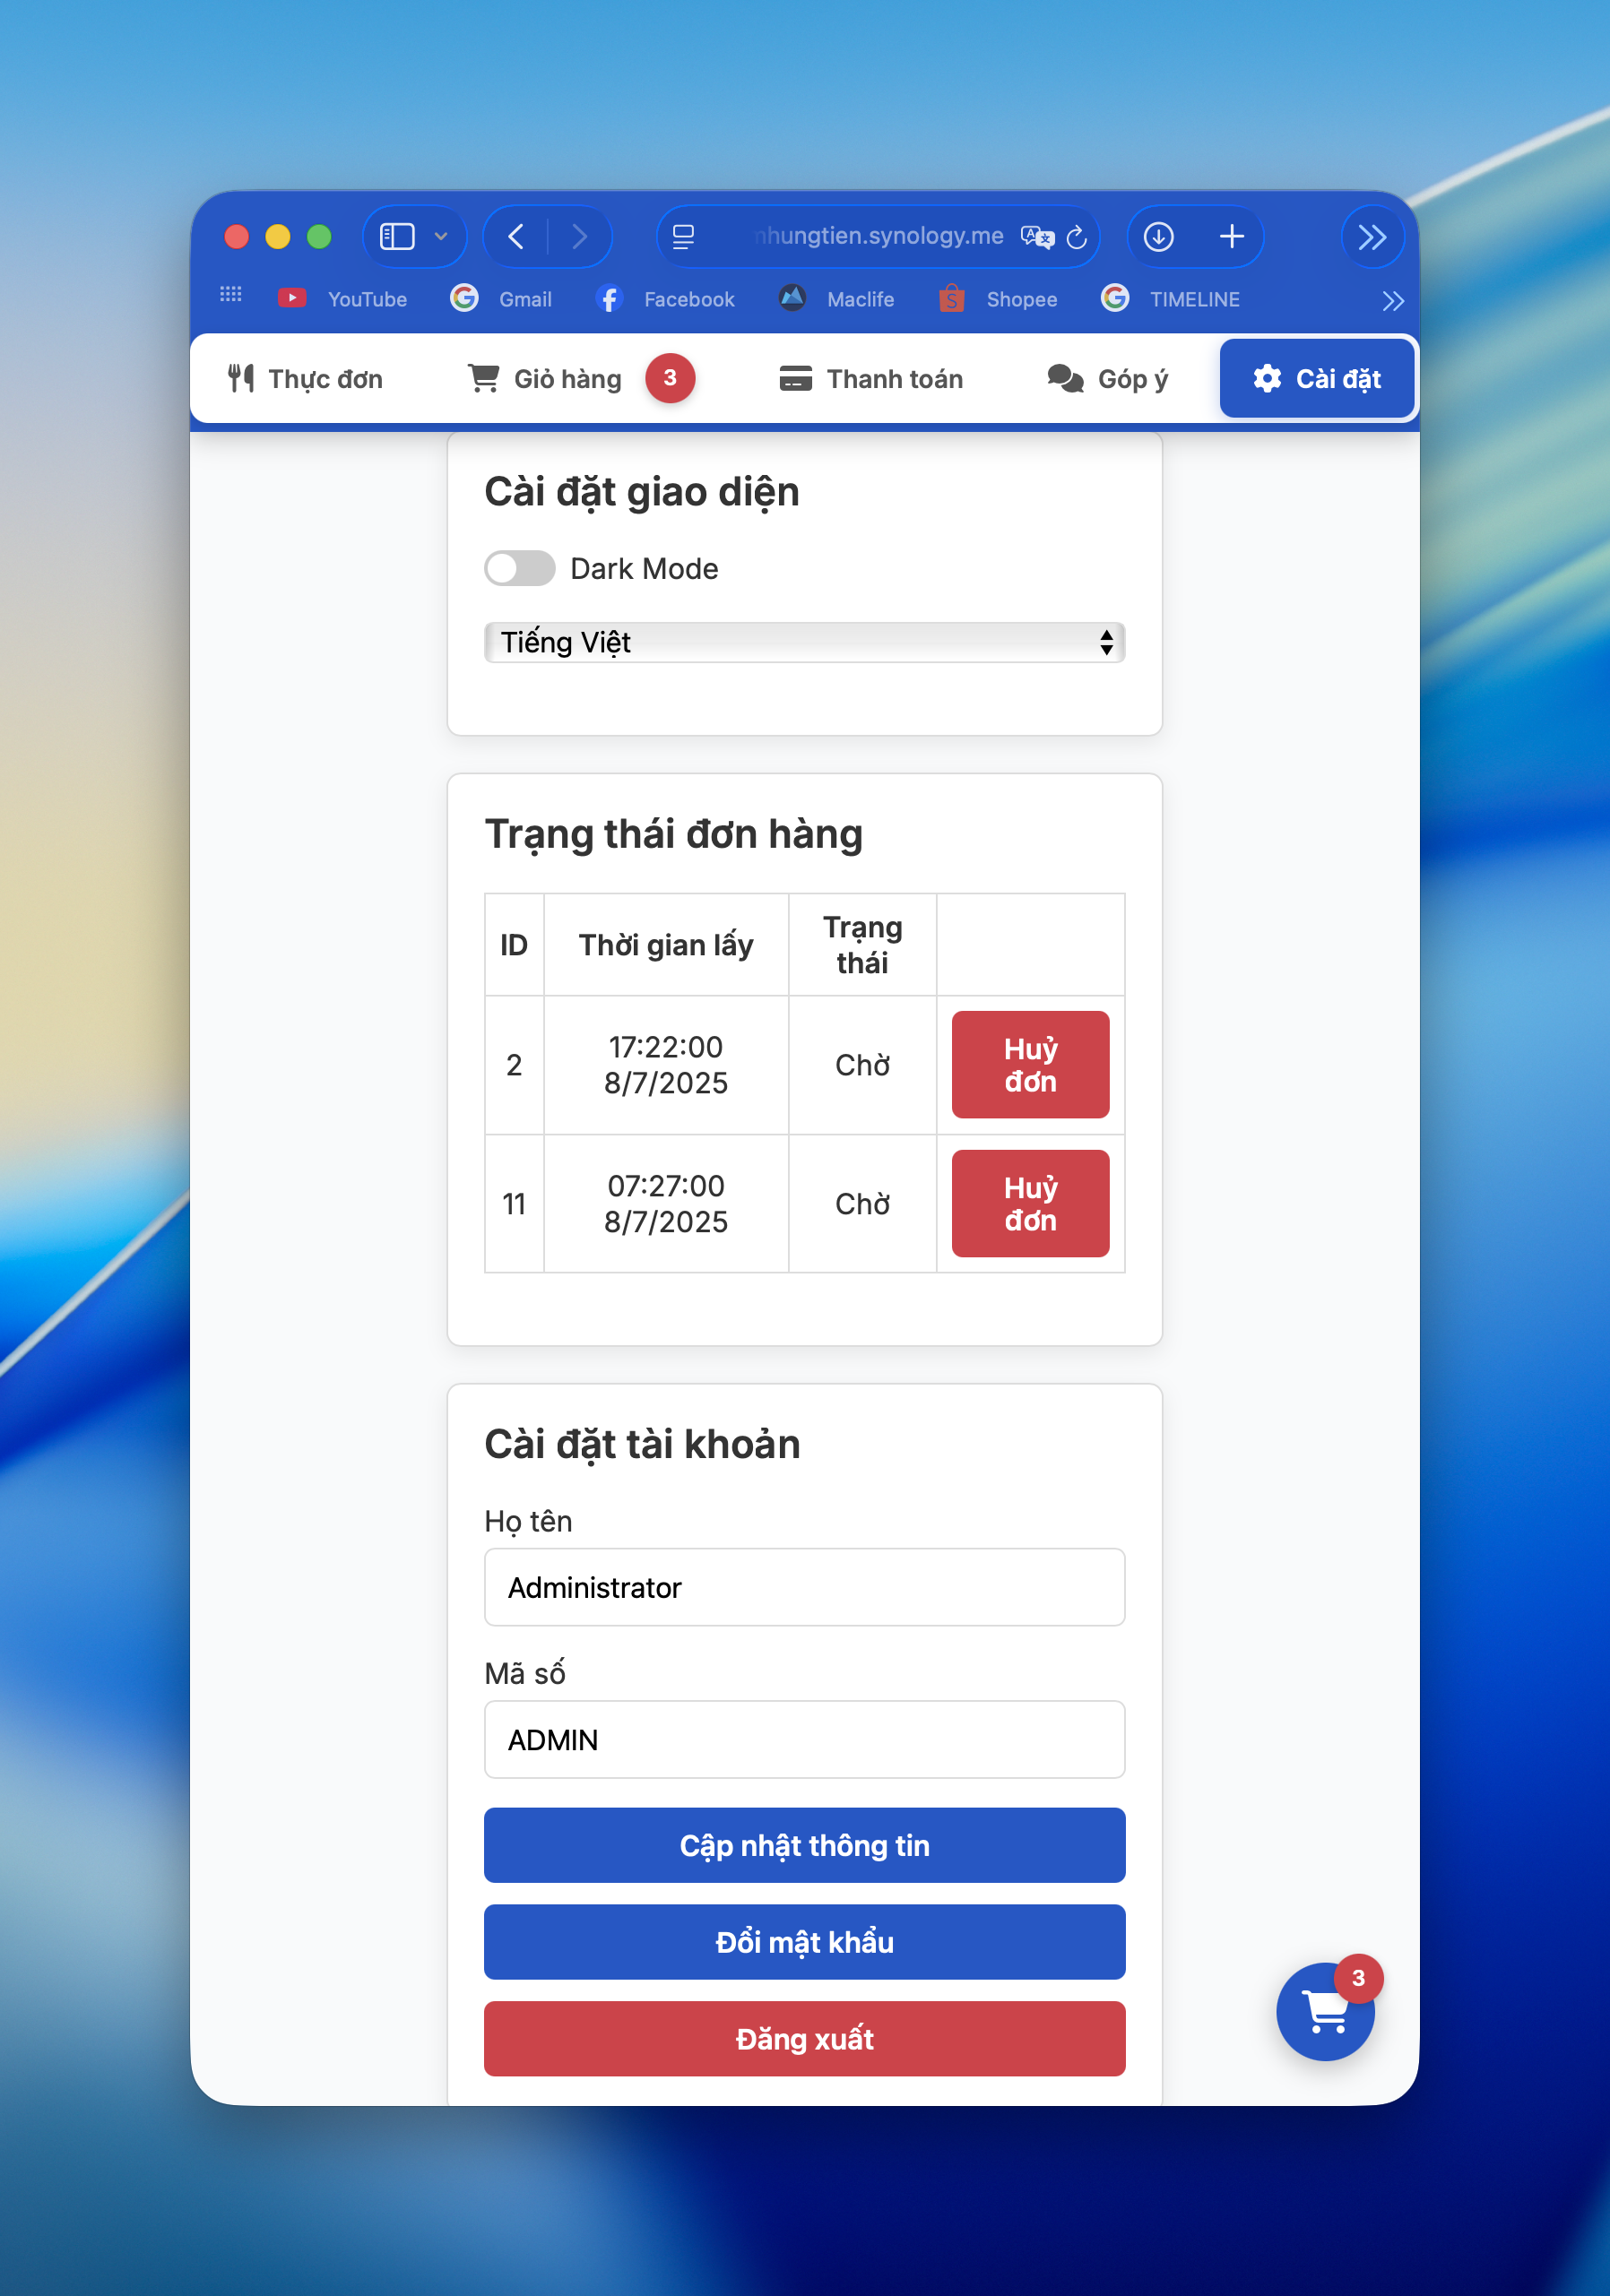
\includegraphics[width=0.9\textwidth]{../figures/ui_user_cai_dat_tai_khoan.png} % Thay thế bằng tên file ảnh của bạn
    \caption{Giao diện cài đặt tài khoản người dùng}
    \label{fig:ui_user_settings}
\end{figure}
\end{itemize}

\subsubsection{Dành cho quản trị viên}
\begin{itemize}[leftmargin=1cm]
    \item \textbf{Quản lý thực đơn}:
        \begin{itemize}[leftmargin=0.5cm]
            \item Thêm/sửa/xóa món ăn
            \item Tải lên hình ảnh và mô hình 3D cho chế độ AR
            \item Quản lý danh mục (Món ăn, Đồ uống, Món tráng miệng)
        \end{itemize}
\begin{figure}[H]
    \centering
    \includegraphics[width=0.9\textwidth]{../figures/ui_admin_quan_ly_thuc_don.png} % Thay thế bằng tên file ảnh của bạn
    \caption{Giao diện quản lý thực đơn của quản trị viên}
    \label{fig:ui_admin_menu}
\end{figure}

    \item \textbf{Quản lý đơn hàng}:
        \begin{itemize}[leftmargin=0.5cm]
            \item Xem danh sách đơn hàng theo thời gian thực
            \item Cập nhật trạng thái đơn hàng
            \item Hủy đơn hàng khi cần thiết
        \end{itemize}
\begin{figure}[H]
    \centering
    \includegraphics[width=0.9\textwidth]{../figures/ui_admin_quan_ly_don_hang.png} % Thay thế bằng tên file ảnh của bạn
    \caption{Giao diện quản lý đơn hàng của quản trị viên}
    \label{fig:ui_admin_orders}
\end{figure}

    \item \textbf{Báo cáo và phân tích}:
        \begin{itemize}[leftmargin=0.5cm]
            \item Thống kê doanh thu theo khoảng thời gian tùy chọn
            \item Phân tích xu hướng đặt món
            \item Báo cáo hiệu suất hoạt động
        \end{itemize}
\begin{figure}[H]
    \centering
    \includegraphics[width=0.9\textwidth]{../figures/ui_admin_bao_cao_doanh_thu.png} % Thay thế bằng tên file ảnh của bạn
    \caption{Giao diện báo cáo doanh thu và phân tích của quản trị viên}
    \label{fig:ui_admin_revenue}
\end{figure}

    \item \textbf{Quản lý người dùng}:
        \begin{itemize}[leftmargin=0.5cm]
            \item Xem và chỉnh sửa thông tin tài khoản người dùng
            \item Quản lý quyền truy cập
        \end{itemize}
\begin{figure}[H]
    \centering
    \includegraphics[width=0.9\textwidth]{../figures/ui_admin_quan_ly_nguoi_dung.png} % Thay thế bằng tên file ảnh của bạn
    \caption{Giao diện quản lý người dùng của quản trị viên}
    \label{fig:ui_admin_users}
\end{figure}
\end{itemize}

\section{Mục tiêu của dự án}

\subsection{Mục tiêu đối với người dùng cuối}
\begin{itemize}[leftmargin=1cm]
    \item \textbf{Nâng cao trải nghiệm đặt món}: Cung cấp giao diện hiện đại, trực quan với tính năng AR độc đáo
    \item \textbf{Tối ưu hóa thời gian}: Giảm thiểu thời gian chờ đợi thông qua hệ thống giới hạn đơn hàng thông minh
    \item \textbf{Đa dạng hóa thanh toán}: Hỗ trợ các phương thức thanh toán điện tử phổ biến
    \item \textbf{Tăng cường tương tác}: Cung cấp kênh phản hồi hiệu quả qua đánh giá và góp ý
    \item \textbf{Cá nhân hóa dịch vụ}: Hỗ trợ cài đặt ngôn ngữ, giao diện theo sở thích cá nhân
\end{itemize}

\subsection{Mục tiêu đối với căng tin (quản trị viên)}
\begin{itemize}[leftmargin=1cm]
    \item \textbf{Số hóa quy trình quản lý}: Tự động hóa việc quản lý thực đơn, đơn hàng và doanh thu
    \item \textbf{Tối ưu hóa vận hành}: Giảm quá tải giờ cao điểm, nâng cao hiệu suất phục vụ
    \item \textbf{Hỗ trợ ra quyết định}: Cung cấp báo cáo doanh thu chi tiết và phân tích xu hướng
    \item \textbf{Nâng cao chất lượng dịch vụ}: Thu thập và phân tích phản hồi khách hàng
    \item \textbf{Giảm thiểu sai sót}: Loại bỏ các công việc thủ công, tăng độ chính xác
\end{itemize}

\subsection{Mục tiêu về mặt công nghệ và triển khai}
\begin{itemize}[leftmargin=1cm]
    \item \textbf{Phát triển nền tảng bền vững}: Xây dựng hệ thống ổn định, có khả năng mở rộng
    \item \textbf{Đổi mới công nghệ}: Áp dụng AR hiệu quả trong ngành F\&B
    \item \textbf{Đơn giản hóa triển khai}: Sử dụng cấu trúc JSON dễ dàng cài đặt và quản lý
    \item \textbf{Mẫu hóa giải pháp}: Tạo ra mô hình có thể tùy chỉnh cho các căng tin khác nhau
    \item \textbf{Thúc đẩy chuyển đổi số}: Góp phần hiện đại hóa ngành dịch vụ ăn uống
\end{itemize}

\section{Tính cấp thiết và tính sáng tạo của dự án}

\subsection{Tính cấp thiết}
Trong bối cảnh đô thị hóa và nhịp sống hiện đại, các căng tin truyền thống đang đối mặt với nhiều thách thức cấp thiết:

\subsubsection{Thách thức hiện tại}
\begin{itemize}[leftmargin=1cm]
    \item \textbf{Quá tải giờ cao điểm}: Xếp hàng dài, chờ đợi lâu gây giảm trải nghiệm
    \item \textbf{Quản lý thủ công}: Dẫn đến sai sót, tốn thời gian và khó tổng hợp dữ liệu
    \item \textbf{Thiếu kênh tương tác}: Khó nắm bắt phản hồi và cải thiện chất lượng
    \item \textbf{Trải nghiệm hạn chế}: Thực đơn nhàm chán, thiếu sự đổi mới
    \item \textbf{Chưa tận dụng công nghệ}: Tiềm năng AR và thanh toán điện tử chưa được khai thác
\end{itemize}

\subsubsection{Giải pháp của Smart Canteen AR}
\begin{itemize}[leftmargin=1cm]
    \item \textbf{Tối ưu hóa quy trình}: Giới hạn đơn hàng theo khung giờ, phân bổ khách hàng hợp lý
    \item \textbf{Nâng cao trải nghiệm}: Công nghệ AR cho phép "nhìn thấy" món ăn trước khi đặt
    \item \textbf{Số hóa quản lý}: Công cụ quản trị mạnh mẽ, báo cáo dựa trên dữ liệu
    \item \textbf{Bắt kịp xu thế}: Phù hợp với chuyển đổi số và công nghệ 4.0
\end{itemize}

\subsection{Tính sáng tạo và điểm mới}
Smart Canteen AR mang lại nhiều yếu tố sáng tạo độc đáo:

\subsubsection{Đổi mới công nghệ}
\begin{itemize}[leftmargin=1cm]
    \item \textbf{AR trong F\&B}: Tích hợp thư viện \texttt{<model-viewer>} cho trải nghiệm 3D trực quan
    \item \textbf{Quản lý thông minh}: Giới hạn 5 đơn/15 phút để tối ưu hóa phục vụ
    \item \textbf{Cấu trúc đơn giản}: Sử dụng JSON thay vì CSDL phức tạp, dễ triển khai
    \item \textbf{Thông báo tự động}: Email nhắc nhở với liên kết hủy đơn tiện lợi
\end{itemize}

\subsubsection{Tích hợp toàn diện}
\begin{itemize}[leftmargin=1cm]
    \item \textbf{Thanh toán đa dạng}: MoMo, VietQR đáp ứng xu hướng không tiền mặt
    \item \textbf{Đa ngôn ngữ}: Hỗ trợ Việt/Anh với giao diện thân thiện
    \item \textbf{Phản hồi tương tác}: Hệ thống đánh giá và góp ý trực tiếp
    \item \textbf{Quản lý thống nhất}: Từ thực đơn đến báo cáo doanh thu
\end{itemize}

\section{Mô hình kinh doanh Lean Canvas}

% Nếu bạn vẫn muốn giữ các bảng chi tiết, bạn có thể đặt hình ảnh Lean Canvas tổng quan ở đây và các bảng phía dưới
\begin{table}[H]
\centering
\caption{Mô hình kinh doanh Smart Canteen AR - Phần 1}
\label{tab:lean-canvas-1}
\begin{tabular}{|p{3cm}|p{3cm}|p{3cm}|p{3cm}|}
\hline
\textbf{Đối tác chính} & \textbf{Hoạt động chính} & \textbf{Đề xuất giá trị} & \textbf{Quan hệ KH} \\
\hline
\textbf{Công nghệ:}
\newline \textbullet{} Nền tảng thanh toán
\newline \textbullet{} Dịch vụ Email API
\newline \textbullet{} Hạ tầng Cloud
\newline \textbullet{} Thư viện AR

\textbf{Triển khai:}
\newline \textbullet{} Căng tin đối tác
\newline \textbullet{} Nhà cung cấp 3D &

\textbf{Phát triển:}
\newline \textbullet{} Phát triển nền tảng
\newline \textbullet{} Quản lý AR
\newline \textbullet{} Hỗ trợ kỹ thuật

\textbf{Vận hành:}
\newline \textbullet{} Quản lý hệ thống
\newline \textbullet{} Marketing
\newline \textbullet{} Chăm sóc KH &

\textbf{Người dùng:}
\newline \textbullet{} Đặt món AR
\newline \textbullet{} Thanh toán đa dạng
\newline \textbullet{} Giảm thời gian chờ

\textbf{Căng tin:}
\newline \textbullet{} Quản lý tự động
\newline \textbullet{} Báo cáo doanh thu
\newline \textbullet{} Dễ triển khai &

\textbf{Tự phục vụ:}
\newline \textbullet{} Giao diện thân thiện
\newline \textbullet{} Hệ thống tự động
\newline \textbullet{} Email nhắc nhở

\textbf{Hỗ trợ:}
\newline \textbullet{} Góp ý trực tiếp
\newline \textbullet{} Hỗ trợ kỹ thuật \\
\hline
\end{tabular}
\end{table}

\begin{table}[H]
\centering
\caption{Mô hình kinh doanh Smart Canteen AR - Phần 2}
\label{tab:lean-canvas-2}
\begin{tabular}{|p{3cm}|p{3cm}|p{3cm}|p{3cm}|}
\hline
\textbf{Kênh phân phối} & \textbf{Phân khúc KH} & \textbf{Cấu trúc chi phí} & \textbf{Nguồn doanh thu} \\
\hline
\textbf{Trực tiếp:}
\newline \textbullet{} Nền tảng web
\newline \textbullet{} Hỗ trợ triển khai

\textbf{Gián tiếp:}
\newline \textbullet{} Đối tác căng tin
\newline \textbullet{} Giới thiệu &

\textbf{B2C:}
\newline \textbullet{} Sinh viên
\newline \textbullet{} Nhân viên VP
\newline \textbullet{} Khách thường xuyên

\textbf{B2B:}
\newline \textbullet{} Căng tin trường học
\newline \textbullet{} Căng tin công ty
\newline \textbullet{} Khu công nghiệp &

\textbf{Cố định:}
\newline \textbullet{} Phát triển SP
\newline \textbullet{} Hosting
\newline \textbullet{} Nhân sự

\textbf{Biến đổi:}
\newline \textbullet{} Email API
\newline \textbullet{} Thanh toán
\newline \textbullet{} Marketing &

\textbf{B2B:}
\newline \textbullet{} Phí subscription
\newline \textbullet{} Phí setup
\newline \textbullet{} Hoa hồng

\textbf{B2C:}
\newline \textbullet{} Quảng cáo
\newline \textbullet{} Phí tiện ích \\
\hline
\end{tabular}
\end{table}

\begin{table}[H]
\centering
\caption{Mô hình kinh doanh Smart Canteen AR - Phần 3}
\label{tab:lean-canvas-3}
\begin{tabular}{|p{2.8cm}|p{2.8cm}|p{2.8cm}|p{2.8cm}|p{2.8cm}|} % Adjusted column widths to match source
\hline
\textbf{Đối tác chính} & \textbf{Hoạt động chính} & \textbf{Giải pháp giá trị} & \textbf{Quan hệ KH} & \textbf{Phân khúc KH} \\
\hline
Nền tảng thanh toán & Phát triển nền tảng & Đặt món AR tiện lợi & Giao diện tự phục vụ & Sinh viên, nhân viên VP \\
\hline
Dịch vụ Email API & Quản lý thực đơn & Quản lý tự động & Hỗ trợ trực tiếp & Căng tin trường học \\
\hline
Hạ tầng Cloud & Hỗ trợ kỹ thuật & Giảm thời gian chờ & Góp ý, đánh giá & Khu công nghiệp \\
\hline
\end{tabular}
\end{table}

\begin{table}[H]
\centering
\caption{Mô hình kinh doanh Smart Canteen AR - Phần 4}
\label{tab:lean-canvas-4}
\begin{tabular}{|p{5cm}|p{5cm}|p{5cm}|}
\hline
\textbf{Nguồn lực chính} & \textbf{Cấu trúc chi phí} & \textbf{Dòng doanh thu} \\
\hline
Đội ngũ phát triển (Frontend, Backend, AR) & Chi phí phát triển \& bảo trì phần mềm & \textbf{B2B (Căng tin):} Phí subscription, hoa hồng đơn hàng \\
\hline
Kiến thức chuyên môn (React, Node.js, AR) & Chi phí hosting \& dịch vụ Email API & \textbf{B2C (Người dùng):} Quảng cáo, phí tiện ích \\
\hline
Mã nguồn hệ thống hoàn chỉnh & Chi phí tích hợp thanh toán & \textbf{Dịch vụ mở rộng:} Tư vấn triển khai \\
\hline
Tài liệu \& thư viện 3D mẫu & Chi phí marketing \& vận hành & \textbf{Đối tác:} Hoa hồng từ thanh toán \\
\hline
\end{tabular}
\end{table}


\section{Kế hoạch thực hiện}

\subsection{Phân tích thị trường}

\subsubsection{Xác định chân dung khách hàng}
Để đảm bảo dự án phát triển đúng hướng và đáp ứng tối đa nhu cầu thị trường, việc xác định rõ chân dung khách hàng là cực kỳ quan trọng.
\begin{itemize}[label=\textbullet]
    \item \textbf{Khách hàng là người dùng cuối (Consumer - B2C):}
    \begin{itemize}[label=\textendash]
        \item \textbf{Đối tượng:} Sinh viên, nhân viên văn phòng, công nhân, khách thăm tại các trường học, khu công nghiệp, công sở, bệnh viện.
        \item \textbf{Đặc điểm nhân khẩu học:} Độ tuổi đa dạng, từ 18-50 tuổi. Trình độ học vấn từ phổ thông đến đại học/sau đại học. Thu nhập trung bình đến ổn định, có khả năng chi trả cho bữa ăn hàng ngày.
        \item \textbf{Thói quen \& sở thích:} Ưu tiên sự tiện lợi, nhanh chóng, và trải nghiệm không rườm rà. Thường xuyên sử dụng điện thoại thông minh và các ứng dụng di động. Sẵn lòng thử nghiệm công nghệ mới (AR, thanh toán không tiền mặt). Quan tâm đến chất lượng, sự đa dạng của món ăn và các chương trình khuyến mãi.
        \item \textbf{Nỗi đau (Pain Points):}
        \begin{itemize}[label=\textrightarrow]
            \item Mất thời gian chờ đợi xếp hàng lâu vào giờ cao điểm.
            \item Khó khăn trong việc xem thực đơn rõ ràng, thiếu thông tin chi tiết về món ăn.
            \item Hạn chế về phương thức thanh toán (chủ yếu tiền mặt).
            \item Thiếu kênh phản hồi trực tiếp và hiệu quả với căng tin.
            \item Không thể xem trước món ăn một cách trực quan.
        \end{itemize}
    \end{itemize}

    \item \textbf{Khách hàng là doanh nghiệp/tổ chức (Business - B2B):}
    \begin{itemize}[label=\textendash]
        \item \textbf{Đối tượng:} Ban quản lý căng tin, chủ nhà ăn, bộ phận hành chính tại các trường học, khu công nghiệp, bệnh viện, doanh nghiệp.
        \item \textbf{Đặc điểm:} Mong muốn hiện đại hóa quy trình, tối ưu hóa chi phí vận hành. Có nhu cầu quản lý chặt chẽ thực đơn, đơn hàng và doanh thu. Quan tâm đến việc nâng cao sự hài lòng của người dùng cuối.
        \item \textbf{Nỗi đau (Pain Points):}
        \begin{itemize}[label=\textrightarrow]
            \item Quá tải trong khâu phục vụ và quản lý đơn hàng thủ công.
            \item Khó khăn trong việc theo dõi doanh thu và phân tích hiệu quả kinh doanh.
            \item Thiếu công cụ quản lý thực đơn linh hoạt (thêm/sửa/xóa món, cập nhật giá).
            \item Không có hệ thống thu thập và phân tích phản hồi khách hàng hiệu quả.
            \item Chi phí vận hành cao do quy trình chưa được số hóa.
        \end{itemize}
    \end{itemize}
\end{itemize}

\subsubsection{Xác định thị trường}
Thị trường mục tiêu của Smart Canteen AR được định nghĩa qua mô hình Bull's Eye Chart, giúp xác định các phân khúc thị trường có tiềm năng nhất và chiến lược tiếp cận phù hợp:

\begin{itemize}[label=\textbullet]
    \item \textbf{Total Addressable Market (TAM) - Thị trường tổng thể có thể phục vụ:} Toàn bộ thị trường dịch vụ ăn uống tại chỗ (Food \& Beverage - F\&B) tại Việt Nam, bao gồm tất cả các loại hình nhà hàng, quán ăn, chuỗi cửa hàng thức ăn nhanh, quán cà phê, và đặc biệt là các căng tin trong mọi loại hình tổ chức (trường học, bệnh viện, nhà máy, văn phòng).
    \begin{itemize}[label=\textendash]
        \item \textit{Dự kiến tăng trưởng hàng năm:} Ngành F\&B Việt Nam duy trì tốc độ tăng trưởng ổn định, với dự báo khoảng 10-15\% mỗi năm (cần nghiên cứu số liệu cụ thể từ các báo cáo thị trường gần nhất để đưa số liệu chính xác).
    \end{itemize}
    \item \textbf{Target Market - Thị trường mục tiêu:} Tập trung vào phân khúc căng tin/nhà ăn nội bộ của các tổ chức lớn như:
    \begin{itemize}[label=\textendash]
        \item \textbf{Căng tin trường học:} Các trường Đại học, Cao đẳng, THPT có quy mô lớn.
        \item \textbf{Căng tin bệnh viện:} Các bệnh viện công và tư lớn, có nhu cầu phục vụ số lượng lớn cán bộ, y bác sĩ, bệnh nhân và người nhà.
        \item \textbf{Căng tin khu công nghiệp/nhà máy:} Các nhà máy, khu công nghiệp với lượng lớn công nhân viên.
        \item \textbf{Căng tin văn phòng/tòa nhà:} Các tòa nhà văn phòng, trụ sở công ty lớn.
        \item \textit{Dự kiến tăng trưởng hàng năm:} Phân khúc này có tiềm năng tăng trưởng bền vững, ước tính 8-12\% do nhu cầu hiện đại hóa và tối ưu hóa vận hành ngày càng cao.
    \end{itemize}
    \item \textbf{Target Segment - Phân khúc mục tiêu (Thị trường trọng điểm):} Các căng tin/đơn vị quản lý muốn hiện đại hóa toàn diện, sẵn sàng áp dụng công nghệ mới và có ngân sách để đầu tư vào giải pháp thông minh. Đặc biệt là những đơn vị:
    \begin{itemize}[label=\textendash]
        \item Đối mặt với vấn đề quá tải vào giờ cao điểm và mong muốn cải thiện trải nghiệm khách hàng.
        \item Đang tìm kiếm một giải pháp quản lý thực đơn, đơn hàng, và doanh thu hiệu quả, giảm thiểu công việc thủ công.
        \item Sẵn sàng tích hợp các phương thức thanh toán điện tử.
        \item Ưu tiên sự khác biệt hóa bằng công nghệ tiên tiến như AR.
        \item \textit{Dự kiến tăng trưởng hàng năm:} Đây là phân khúc có tốc độ tăng trưởng nhanh nhất trong thị trường căng tin, có thể đạt 15-20\% hoặc hơn khi các giải pháp công nghệ trở nên phổ biến hơn.
    \end{itemize}
    \item \textbf{Market Share - Thị phần:} Tỷ lệ phần trăm các căng tin trong phân khúc mục tiêu mà Smart Canteen AR đã tiếp cận và triển khai thành công. Đây là mục tiêu mà dự án cần đạt được trong các giai đoạn phát triển.
    \begin{itemize}[label=\textendash]
        \item \textit{Mục tiêu ngắn hạn (1 năm):} Chiếm 1-2\% thị phần phân khúc trọng điểm.
        \item \textit{Mục tiêu trung hạn (3 năm):} Chiếm 5-10\% thị phần phân khúc trọng điểm.
    \end{itemize}
\end{itemize}

\subsubsection{Các xu thế hiện nay trên thị trường có lợi cho dự án của bạn:}

\begin{itemize}[label=\textbullet]
    \item \textbf{Sự bùng nổ của chuyển đổi số:} Các doanh nghiệp và tổ chức đang đẩy mạnh ứng dụng công nghệ để tối ưu hóa quy trình, nâng cao hiệu quả hoạt động và tăng cường trải nghiệm khách hàng. Ngành F\&B không nằm ngoài xu hướng này.
    \item \textbf{Phát triển mạnh mẽ của thanh toán không tiền mặt:} Sự phổ biến của ví điện tử (Momo, ZaloPay), mobile banking, và mã QR (VietQR) đã thay đổi thói quen thanh toán của người tiêu dùng, tạo điều kiện thuận lợi cho các hệ thống đặt món trực tuyến.
    \item \textbf{Nhu cầu về sự tiện lợi và nhanh chóng:} Nhịp sống hiện đại khiến người tiêu dùng ngày càng ưu tiên các dịch vụ tiết kiệm thời gian, giảm thiểu sự chờ đợi.
    \item \textbf{Sự trưởng thành của công nghệ AR/VR:} Công nghệ thực tế tăng cường (AR) đã và đang được tích hợp vào nhiều lĩnh vực, mang lại trải nghiệm mới lạ, trực quan và hấp dẫn, thu hút sự chú ý của người dùng.
    \item \textbf{Xu hướng cá nhân hóa và tương tác khách hàng:} Người tiêu dùng muốn được lắng nghe, muốn có khả năng đánh giá và góp ý trực tiếp về sản phẩm/dịch vụ để cảm thấy được trân trọng và góp phần cải thiện chất lượng.
    \item \textbf{Tập trung vào hiệu quả vận hành:} Các căng tin ngày càng chú trọng đến việc tối ưu hóa quy trình nội bộ, giảm thiểu lãng phí và tăng cường năng suất.
\end{itemize}

\subsubsection{Đối thủ cạnh tranh:}
Thị trường cung cấp giải pháp cho ngành F\&B khá sôi động, Smart Canteen AR sẽ cạnh tranh với:

\begin{itemize}[label=\textbullet]
    \item \textbf{Các nền tảng đặt món và giao hàng trực tuyến lớn:} GrabFood, ShopeeFood, Baemin, GoFood. Tuy nhiên, các nền tảng này chủ yếu tập trung vào giao hàng từ các nhà hàng bên ngoài, ít chuyên biệt cho mô hình căng tin nội bộ và không tích hợp AR.
    \item \textbf{Các phần mềm quản lý nhà hàng/POS truyền thống:} KiotViet, Sapo POS, iPOS. Các giải pháp này mạnh về quản lý kinh doanh tổng thể nhưng thường thiếu tính năng đặt món trực tuyến cho người dùng cuối và không có tính năng AR.
    \item \textbf{Các ứng dụng đặt món nội bộ đơn giản:} Một số trường học hoặc công ty có thể tự phát triển các ứng dụng đặt món cơ bản, nhưng thường hạn chế về tính năng, trải nghiệm người dùng và công nghệ (thiếu AR, thanh toán đa dạng).
    \item \textbf{Hình thức đặt món truyền thống:} Đặt trực tiếp tại quầy, order giấy.
\end{itemize}

\textbf{Lợi thế cạnh tranh của Smart Canteen AR:}

\begin{itemize}[label=\textbullet]
    \item \textbf{Điểm khác biệt cốt lõi:} Tập trung chuyên biệt vào mô hình căng tin với tính năng AR độc đáo và cơ chế giới hạn đơn hàng thông minh.
    \item \textbf{Dễ triển khai:} Cấu trúc dữ liệu JSON giúp triển khai nhanh chóng, phù hợp với các căng tin muốn thử nghiệm giải pháp số mà không cần hạ tầng phức tạp.
    \item \textbf{Trải nghiệm người dùng vượt trội:} Giao diện trực quan, thanh toán tiện lợi và thông báo tự động.
\end{itemize}

\subsubsection{Nhà cung cấp:}
Để hệ thống Smart Canteen AR hoạt động hiệu quả, chúng tôi sẽ hợp tác với các nhà cung cấp sau:

\begin{itemize}[label=\textbullet]
    \item \textbf{Nhà cung cấp dịch vụ hạ tầng đám mây/hosting:} AWS, Google Cloud, Microsoft Azure, hoặc các nhà cung cấp local để lưu trữ máy chủ và dữ liệu, đảm bảo hệ thống hoạt động ổn định và có khả năng mở rộng.
    \item \textbf{Nhà cung cấp dịch vụ Email API (SMTP):} SendGrid, Mailgun, AWS SES để đảm bảo việc gửi email xác nhận tài khoản và nhắc nhở đơn hàng được thực hiện nhanh chóng, đáng tin cậy. (Mặc định đang dùng \texttt{canteenar@gmail.com} nhưng cần chuyển sang dịch vụ chuyên nghiệp khi mở rộng).
    \item \textbf{Các đối tác cổng thanh toán:} MoMo, ZaloPay, các ngân hàng hỗ trợ VietQR để tích hợp đa dạng phương thức thanh toán trực tuyến, mang lại sự tiện lợi tối đa cho người dùng.
    \item \textbf{Nhà cung cấp công cụ và thư viện phát triển:} Nền tảng Node.js, thư viện React, \texttt{<model-viewer>} (mã nguồn mở, nhưng cần hỗ trợ kỹ thuật nếu gặp vấn đề phức tạp).
    \item \textbf{Nhà cung cấp dịch vụ thiết kế 3D (nếu có):} Trong trường hợp các căng tin không có sẵn mô hình 3D cho món ăn, chúng tôi có thể hợp tác với các đối tác thiết kế để tạo ra các mô hình chất lượng cao.
\end{itemize}

\subsubsection{Sản phẩm thay thế:}
Các sản phẩm/phương thức có thể thay thế Smart Canteen AR trong bối cảnh hiện tại bao gồm:

\begin{itemize}[label=\textbullet]
    \item \textbf{Đặt món trực tiếp tại quầy căng tin:} Đây là phương thức truyền thống, đơn giản nhưng thường gây ra tình trạng chờ đợi và thiếu sự thuận tiện.
    \item \textbf{Tự chuẩn bị bữa ăn từ nhà:} Đối với một số người dùng, việc mang theo đồ ăn từ nhà là lựa chọn thay thế để tiết kiệm chi phí hoặc vì lý do sức khỏe.
    \item \textbf{Đặt đồ ăn từ các ứng dụng giao hàng bên ngoài:} Người dùng có thể đặt món từ các nhà hàng bên ngoài thông qua GrabFood, ShopeeFood nếu căng tin không phải là lựa chọn duy nhất hoặc không có dịch vụ tốt.
    \item \textbf{Các hệ thống đặt món qua điện thoại/tin nhắn:} Một số căng tin có thể nhận đơn qua điện thoại hoặc tin nhắn Zalo, nhưng thiếu tính năng quản lý tự động và trực quan.
    \textbf{Các ứng dụng đặt món nội bộ cơ bản:} Một số tổ chức có thể phát triển các ứng dụng rất đơn giản chỉ với chức năng đặt món cơ bản, thiếu các tính năng nâng cao như AR, quản lý chi tiết, hoặc thanh toán tích hợp.
\end{itemize}

\subsection{Kế hoạch phát triển sản phẩm}

Kế hoạch phát triển sản phẩm Smart Canteen AR sẽ được chia thành các giai đoạn cụ thể nhằm đảm bảo tiến độ, chất lượng và khả năng mở rộng trong tương lai.
\begin{itemize}[label=\textbullet]
    \item \textbf{Giai đoạn 1: Phát triển phiên bản MVP (Minimum Viable Product) - Quý 3/2025}
    \begin{itemize}[label=\textendash]
        \item \textbf{Mục tiêu:} Hoàn thiện các chức năng cốt lõi để hệ thống có thể hoạt động và giải quyết các vấn đề cấp thiết nhất.
        \item \textbf{Các công việc chính:}
        \begin{itemize}[label=\textrightarrow]
            \item Phát triển hệ thống đăng ký, đăng nhập và xác thực người dùng (email xác nhận, quên/đổi mật khẩu).
            \item Xây dựng giao diện xem thực đơn, thêm món vào giỏ hàng và đặt món.
            \item Triển khai cơ chế giới hạn 5 đơn hàng/khung 15 phút.
            \item Tích hợp thanh toán Momo và VietQR.
            \item Phát triển tính năng AR cơ bản: cho phép tải lên và hiển thị mô hình 3D món ăn.
            \item Hoàn thiện các chức năng quản trị viên: quản lý thực đơn (thêm, sửa, xóa, tải ảnh, tải 3D model), xem danh sách đơn hàng.
            \item Xây dựng cấu trúc thư mục và dữ liệu JSON ban đầu.
        \end{itemize}
        \item \textbf{Kết quả mong đợi:} Một hệ thống hoạt động ổn định, sẵn sàng để triển khai thử nghiệm nội bộ hoặc tại một căng tin mẫu.
    \end{itemize}

    \item \textbf{Giai đoạn 2: Thử nghiệm, Thu thập phản hồi và Cải tiến - Quý 4/2025}
    \begin{itemize}[label=\textendash]
        \item \textbf{Mục tiêu:} Đánh giá hiệu quả của MVP, thu thập ý kiến từ người dùng thực tế và hoàn thiện sản phẩm dựa trên phản hồi.
        \item \textbf{Các công việc chính:}
        \begin{itemize}[label=\textrightarrow]
            \item Triển khai thử nghiệm tại 1-2 căng tin đối tác (ví dụ: căng tin trường Đại học Khoa học Tự nhiên).
            \item Thiết lập kênh thu thập phản hồi từ người dùng cuối (mục "Góp ý", đánh giá món ăn) và quản trị viên.
            \item Phân tích dữ liệu sử dụng và phản hồi để xác định các điểm cần cải thiện, lỗi hệ thống.
            \item Tối ưu hóa hiệu suất hệ thống, sửa lỗi và nâng cao trải nghiệm người dùng (UI/UX).
            \item Cải thiện quy trình gửi email nhắc nhở và quản lý hủy đơn.
            \item Phát triển chức năng báo cáo doanh thu theo khoảng thời gian tùy chọn cho quản trị viên.
        \end{itemize}
        \item \textbf{Kết quả mong đợi:} Sản phẩm được cải thiện đáng kể về tính năng và trải nghiệm, sẵn sàng cho giai đoạn mở rộng.
    \end{itemize}

    \item \textbf{Giai đoạn 3: Mở rộng tính năng và Tối ưu hóa - Quý 1-2/2026}
    \begin{itemize}[label=\textendash]
        \item \textbf{Mục tiêu:} Nâng cấp sản phẩm với các tính năng tiên tiến, tăng cường khả năng mở rộng và đáp ứng nhu cầu đa dạng hơn.
        \item \textbf{Các công việc chính:}
        \begin{itemize}[label=\textrightarrow]
            \item Phát triển tính năng quản lý người dùng chi tiết (phân quyền, chỉnh sửa thông tin).
            \item Nâng cấp báo cáo doanh thu với các biểu đồ trực quan, phân tích xu hướng, và các chỉ số kinh doanh quan trọng khác.
            \item Nghiên cứu và tích hợp thêm các phương thức thanh toán phổ biến khác (nếu có nhu cầu).
            \item Xây dựng hệ thống thông báo đẩy (push notification) cho người dùng cuối (nếu phát triển ứng dụng di động).
            \item Cá nhân hóa trải nghiệm người dùng (gợi ý món ăn dựa trên lịch sử đặt hàng, sở thích).
            \item Cải thiện khả năng quản lý mô hình 3D và hình ảnh (tối ưu dung lượng, chất lượng hiển thị).
            \item Xem xét tích hợp với hệ thống quản lý kho nguyên liệu của căng tin (tùy chọn).
        \end{itemize}
        \item \textbf{Kết quả mong đợi:} Một nền tảng mạnh mẽ, đa năng, có khả năng cạnh tranh cao trên thị trường.
    \end{itemize}

    \item \textbf{Giai đoạn 4: Hoàn thiện, Thương mại hóa và Mở rộng thị trường - Từ Quý 3/2026}
    \begin{itemize}[label=\textbullet]
        \item \textbf{Mục tiêu:} Đưa sản phẩm ra thị trường rộng rãi, xây dựng thương hiệu và thiết lập mô hình kinh doanh bền vững.
        \item \textbf{Các công việc chính:}
        \begin{itemize}[label=\textrightarrow]
            \item Hoàn thiện tài liệu hướng dẫn sử dụng chi tiết cho cả người dùng cuối và quản trị viên.
            \item Xây dựng chính sách bảo mật, điều khoản sử dụng và hợp đồng dịch vụ.
            \item Phát triển chiến lược marketing và bán hàng để tiếp cận các căng tin tiềm năng.
            \item Thiết lập đội ngũ hỗ trợ khách hàng và quy trình bảo trì, cập nhật hệ thống.
            \item Nghiên cứu và triển khai các gói dịch vụ (phí đăng ký, hoa hồng trên đơn hàng, gói tính năng cao cấp) để tạo dòng doanh thu.
            \item Mở rộng thị trường sang các khu vực địa lý khác hoặc phân khúc căng tin mới.
            \item Tiếp tục nghiên cứu và phát triển các tính năng đột phá dựa trên xu hướng công nghệ.
        \end{itemize}
        \item \textbf{Kết quả mong đợi:} Smart Canteen AR trở thành giải pháp hàng đầu cho căng tin thông minh, có vị thế vững chắc trên thị trường.
    \end{itemize}

\section{Phân tích rủi ro và biện pháp giảm thiểu}
\begin{riskbox}
\begin{itemize}
    \item \textbf{Rủi ro kỹ thuật}: Công nghệ AR và thanh toán trực tuyến có thể
    phát sinh lỗi khi vận hành ở quy mô lớn. \textit{Biện pháp:} thử nghiệm diện
    rộng, áp dụng quy trình kiểm thử chặt chẽ và có phương án dự phòng.
    \item \textbf{Rủi ro thị trường}: Người dùng còn mới lạ với AR hoặc thói quen
    đặt món truyền thống. \textit{Biện pháp:} tăng cường hoạt động truyền thông
    và hướng dẫn, đưa ra chính sách khuyến khích sử dụng ban đầu.
    \item \textbf{Rủi ro vận hành}: Quá trình tích hợp với căng tin hiện hữu có thể
    gặp khó khăn về hạ tầng hoặc nhân lực. \textit{Biện pháp:} xây dựng tài liệu
    hướng dẫn chi tiết, đào tạo nhân viên và hỗ trợ kỹ thuật kịp thời.
    \item \textbf{Rủi ro tài chính}: Chi phí duy trì hạ tầng, quảng bá có thể vượt
    dự toán. \textit{Biện pháp:} lập ngân sách dự phòng và theo dõi sát sao các
    chỉ số tài chính qua từng giai đoạn.
\end{itemize}
\end{riskbox}

\section{Kết luận}
Smart Canteen AR là giải pháp tiên phong ứng dụng thực tế tăng cường trong lĩnh
vực căng tin thông minh. Dự án hướng tới nâng cao trải nghiệm người dùng, tối ưu
quy trình vận hành và mở ra cơ hội chuyển đổi số mạnh mẽ cho ngành F\&B. Với kế
hoạch phát triển bài bản cùng các biện pháp giảm thiểu rủi ro, nhóm tin tưởng dự
án sẽ đạt được thành công bền vững trong tương lai.

\clearpage % Bắt đầu trang mới cho tài liệu tham khảo
\section{Tài liệu tham khảo}
\begin{thebibliography}{99} % 99 là độ rộng tối đa của số thứ tự (ví dụ: 1-99)
    \bibitem{hiep_hoi_nha_hang_2024}
    Hiệp hội Nhà hàng Việt Nam. (2024). \textit{Báo cáo thường niên Thị trường F\&B Việt Nam 2023-2024}. Hà Nội: Nhà xuất bản Thống kê.
    \bibitem{bo_ke_hoach_2023}
    Bộ Kế hoạch và Đầu tư. (2023). \textit{Chiến lược quốc gia về chuyển đổi số đến năm 2025, định hướng đến năm 2030}. Hà Nội: Cổng thông tin Chính phủ.

    \bibitem{google_model_viewer_2024}
    Google Developers. (2024). \textit{\texttt{<model-viewer>} Documentation}. Truy cập từ: \url{https://modelviewer.dev/}

    \bibitem{react_doc_2024}
    React Documentation. (2024). \textit{Getting Started with React}. Truy cập từ: \url{https://react.dev/learn}

    \bibitem{nodejs_doc_2024}
    Node.js Documentation. (2024). \textit{Node.js API Reference}. Truy cập từ: \url{https://nodejs.org/docs/latest/api/}

    \bibitem{ngan_hang_nha_nuoc_2023}
    Ngân hàng Nhà nước Việt Nam. (2023). \textit{Báo cáo về tình hình thanh toán không dùng tiền mặt tại Việt Nam}. Hà Nội: Ngân hàng Nhà nước Việt Nam.

    \bibitem{deloitte_2023}
    Deloitte. (2023). \textit{The Future of Food Service: Digital Transformation and Emerging Technologies}. Truy cập từ: \url{https://www2.deloitte.com/}

    \bibitem{porter_1985}
    Porter, M. E. (1985). \textit{Competitive Advantage: Creating and Sustaining Superior Performance}. New York: Free Press.

    \bibitem{ries_2011}
    Ries, E. (2011). \textit{The Lean Startup: How Today's Entrepreneurs Use Continuous Innovation to Create Radically Successful Businesses}. Crown Business.
\end{thebibliography}
\end{document}